% 图 1.6 椭球形磁化样品（主轴 a、b、c）
\documentclass[tikz,border=5pt]{standalone}
\usepackage{amsmath}
\usepackage{bm}
\usepackage{fontspec}
\setmainfont{Times New Roman}
\begin{document}
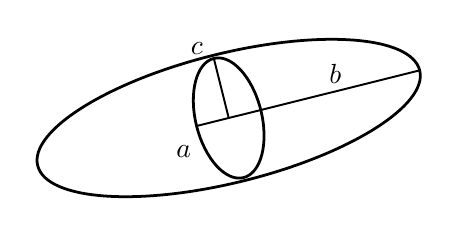
\begin{tikzpicture}[line width=1.0pt]
\begin{scope}[rotate=14]
% 椭球轮廓
\draw (0,0) ellipse (2.5 and 0.82);
% 中央横截面（含 a、c 轴）
\draw (0,0) ellipse (0.42 and 0.78);
% 长半轴 b
\draw[line width=0.7pt] (0,0) -- (2.5,0);
\node at (1.45,0.22) {$b$};
% 短半轴 c（竖直）
\draw[line width=0.7pt] (0,0) -- (0,0.78);
\node at (-0.18,0.95) {$c$};
% 横截面水平半径 a
\draw[line width=0.7pt] (0,0) -- (-0.42,0);
\node at (-0.66,-0.28) {$a$};
\end{scope}
\end{tikzpicture}
\end{document}
